\documentclass{article}
\usepackage{polski}
\usepackage{blindtext}
\usepackage{amsmath}
\usepackage{mathtools}
\usepackage{graphicx} 
\usepackage{wrapfig}
\usepackage{amssymb}
\usepackage{multirow}
\usepackage[usenames,dvipsnames,svgnames,table]{xcolor}
\usepackage{float}
\usepackage[caption = false]{subfig}
\usepackage{caption}
\newcommand\tab[1][1cm]{\hspace*{#1}}
\usepackage[a4paper, left=2cm, right=2cm, top=2cm, bottom=2cm, headsep=1.2cm]{geometry}

\usepackage{titling}
\newcommand{\subtitle}[1]{%
  \posttitle{%
    \par\end{center}
    \begin{center}\large#1\end{center}
    \vskip0.5em}%
}


\begin{document}
\title{Generowanie ciągu liczb pseudolosowych o rozkładzie jednorodnym i trójkątnym}
\author{Wiktoria Zaczyk}
\date{15.06.2020}

\maketitle

\begin{figure}[H]
\begin{center}

\includegraphics[height=0.3\linewidth]{agh.jpg}
\label{pierwszy} 
\end{center}
\end{figure}

\section{Wstęp teoretyczny}
\textbf{Definicja kongruencji}
\newline

\begin{equation}
\begin{array}{c}
a \equiv r\hspace{4} mod \hspace{4}  n \Rightarrow r = a - [\frac{a}{n}]n
\end{array}
\end{equation}

\newline
\setlength{\parindent}{0pt}
\textbf{Rozkład jednomianowy}
\newline
Funkcja gęstości prawdopodobieństwa to $f(x)=(n+1)x^n$ a pozostałe parametry rozkładu przyjmijmy w postaci $x\in [0,1]$, $n=1,2,3, ...$. Określamy funkcję opisującą dystrybuantę:

\begin{equation}
\begin{array}{c}
F(x)=(n+1)\displaystyle \int_{0}^{x} x'^n dx'= (n+1) \frac{x^{n+1}}{n+1}=U
\end{array}
\end{equation}

uzależniamy x od U: $x=U^{\frac{1}{n+1}}$, $x\in [0,1]$



\vspace{5}
\setlength{\parindent}{0pt}
\textbf{Rozkład trójkątny}
\newline
Funkcję gęstości prawdopodobieństwa dla rozkładu trójkątnego opisujemy poniższym wzorem:

\begin{equation}
    f(x:\mu ,\Delta)=-\frac{|x-\mu|}{\Delta^2}+\frac{1}{\Delta}
\end{equation}

gdzie: $\mu$ to środek rozkładu, a $\Delta$ to jego szerokość.
\newline
Dystrybuanta rozkładu trójkątnego:

\begin{equation}
F(a)=P(x<a)=\displaystyle \int_{\mu-\Delta}^{a} f(x:\mu ,\Delta)dx = \left\{ \begin{array}{ll}
-\frac{1}{\Delta^2}(-\frac{x^2}{2}+\mu x)+\frac{x}{\Delta} & \textrm{ $x\leq \mu$}\\
-\frac{1}{\Delta^2}(\frac{x^2}{2}-\mu x+\mu^2)+\frac{x}{\Delta} & \textrm{ $x>\mu$}
\end{array} \right

\end{equation}

Jeśli $\xi_1 \in$  U(0, 1) i $\xi_2 \in$  U(0, 1) to zmienną o rozkładzie trójkątnym oraz parametrach µ i ∆
generujemy stosując formułę:

\begin{equation}
    x=\mu + (\xi_1 + \xi_2 -1) \cdot \Delta
\end{equation}

\section{Cel zadania}

Zadaniem w trakcie laboratoriów było wygenerowanie ciąu liczb pseudolosowyach za pomocą: 

\newline

\setlength{\parindent}{0pt}
\textbf{Rozkład jednorodny}
Startując od $x_0 = 10$ należy wygenerować $n = 10^4$
liczb pseudolosowych przy użyciu generatora
mieszanego: $x_{n+1}=(ax_n+c)$ mod m
\newline
o parametrach (typu long int):
\begin{enumerate}
    \item $a=123$, $m=2^15$
    \item $a=69069$, $m=2^32$
\end{enumerate}
\newline

\setlength{\parindent}{0pt}
\textbf{Rozkład trójkątny}
Następnie należało wygenerować $n= 10^3$
liczb o rozkładzie trójkątnym, zgodnie ze wzorem 
o parametrach $\mu=4$ $\Delta=3$
\newline
Kolejno podzielić przedział $[\mu-\Delta, \mu+\Delta]$ a $K=1$ podprzedziałów i zliczyć ile liczb wpada do każdego z nich.

\newline

Dla rozkładu trójkatnego przeprowadzić test $\chi^
2$ tj. określić wartość statystyki testowej

\begin{equation}
    \chi^2=\sum_{i=1}^K \frac{(n_i-n\cdot p_i)^2}{n\cdot p_i}
\end{equation}
\begin{equation}
    p_i=F(x_{i,max})-F(x_{i,min})
\end{equation}

\newline

\section{Wyniki}
\textbf{I.}

\begin{figure}[H]
\begin{center}
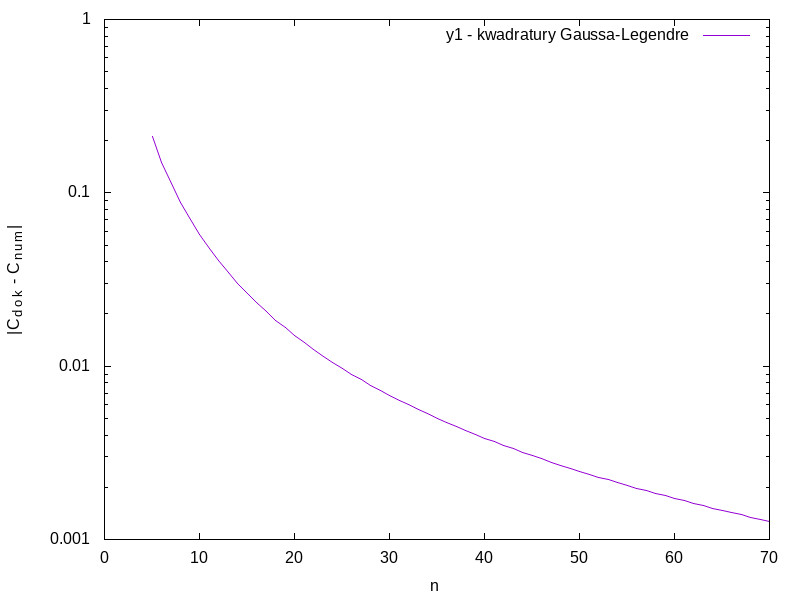
\includegraphics[height=0.5\linewidth]{zad1.jpg}
\caption{Wykres zależności modułu różnicy wartości dokładnej całki, a całki obliczonej numerycznie od ilości przyjętych
węzłów}
\label{pierwszy} 
\end{center}
\end{figure}

Jak można zauważyć na wykresie, wraz ze zwiększeniem liczby węzłów, cały czas
zwiększała się dokładność wyznaczonego przybliżenia wartości całki metodą
kwadratury Gaussa-Legendre’a.

\newpage
\textbf{II.}

\begin{figure}[H]
\begin{center}
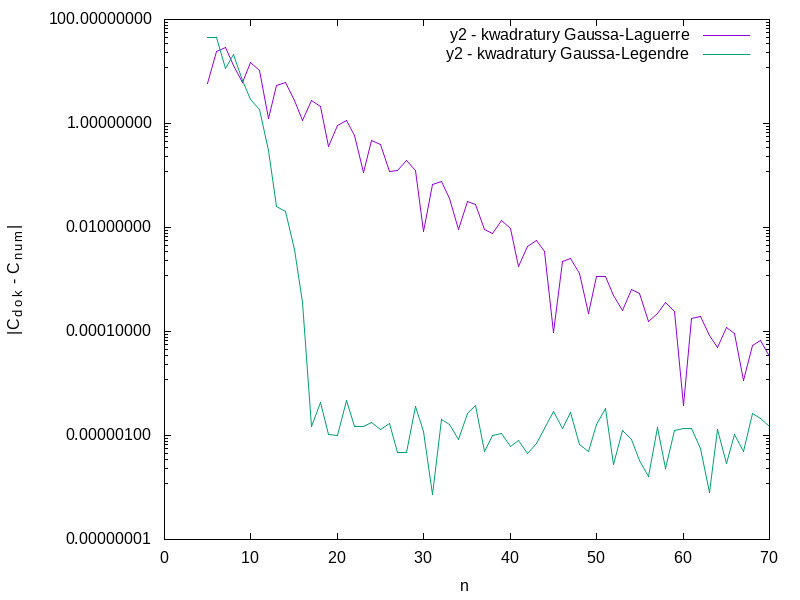
\includegraphics[height=0.5\linewidth]{zad2.jpg}
\caption{Wykres zależności modułu różnicy wartości dokładnej całki, a całki obliczonej numerycznie od ilości przyjętych
węzłów}
\label{pierwszy} 
\end{center}
\end{figure}
\newline
Dla metody kwadratur Gaussa-Legendre’a dokładność stale się zwiększała podczas
zwiększania liczby węzłów. Dla ich większej liczby następowały oscylacje różnicy
rozwiązania dokładnego z numerycznym i jakość wyznaczonego przybliżenia nie
zwiększała się znacznie. Dla metody kwadratur Gaussa-Laguerre’a mimo niewielkich oscylacji, jakość
przybliżenia zwiększała się przy zwiększaniu liczby węzłów do 70.
\newline
\textbf{III.}

\begin{figure}[H]
\begin{center}
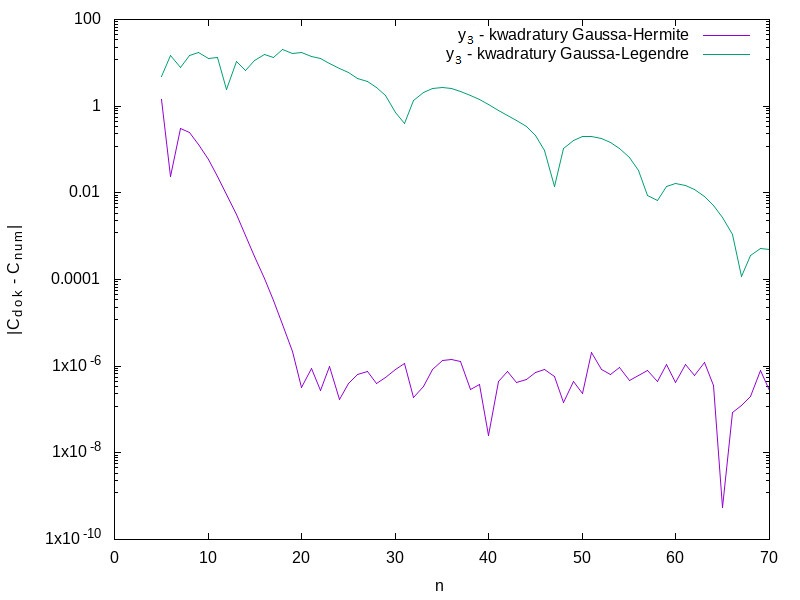
\includegraphics[height=0.5\linewidth]{zad3.jpg}
\caption{Wykres zależności modułu różnicy wartości dokładnej całki, a całki obliczonej numerycznie od ilości przyjętych
węzłów}
\label{pierwszy} 
\end{center}
\end{figure}

Dla metody kwadratur Gaussa-Hermite’a dokładność wyznaczonej wartości całki
oznaczonej III. zwiększała się podobnie jak dokładność przybliżenia całki II. metodą
kwadratur Gaussa-Legendre’a. Dla większej liczby przyjętych węzłów,
występowały oscylacje i dokładność nie zwiększała sie znacząco. Można zauważyć powtarzające się
'uskoki' wykresu, gdzie błąd przybliżenia najpierw rośnie, a następnie zaczyna maleć.
Dla całej dziedziny rozpatrywanej liczby węzłów, metoda kwadratur GaussaHermite’a pozwoliła mi uzyskać lepsze przybliżenie niż metoda kwadratur GaussaLegendre’a.

\textbf{I.}

\begin{figure}[H]
\begin{center}
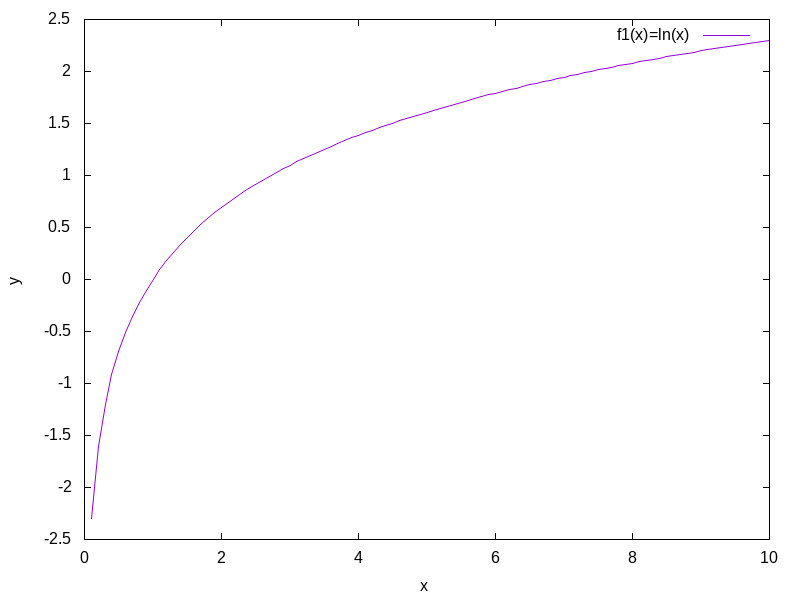
\includegraphics[height=0.5\linewidth]{f1.jpg}
\caption{Wykres iloczynu funkcji podcałkowej i funkcji wagowej$f(x)\cdot p(x)$}
\label{pierwszy} 
\end{center}
\end{figure}

\textbf{II.}

\begin{figure}[H]
\begin{center}
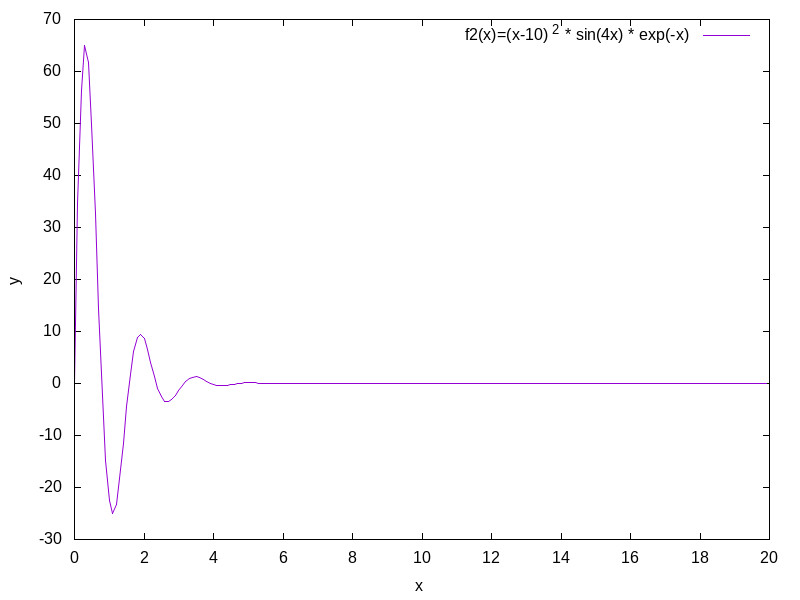
\includegraphics[height=0.5\linewidth]{f2.jpg}
\caption{Wykres iloczynu funkcji podcałkowej i funkcji wagowej$f(x)\cdot p(x)$}
\label{pierwszy} 
\end{center}
\end{figure}
\newpage
\textbf{III.}

\begin{figure}[H]
\begin{center}
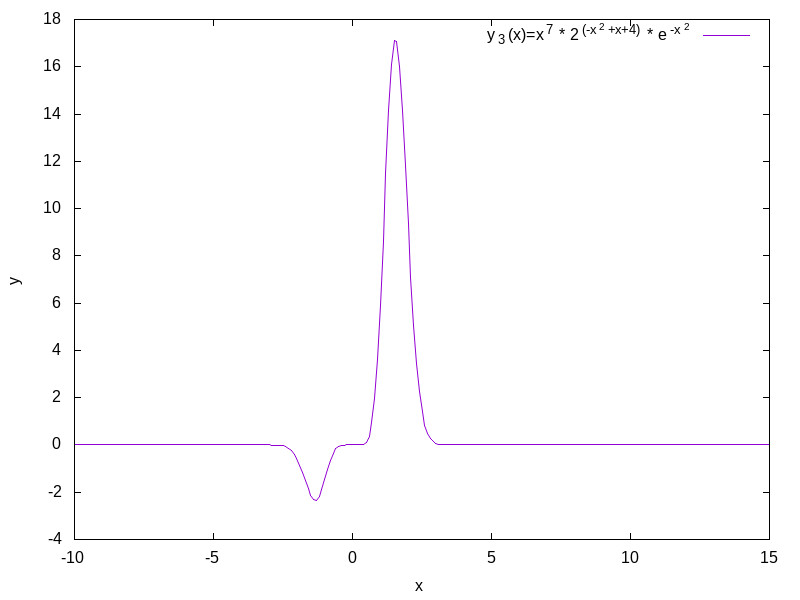
\includegraphics[height=0.5\linewidth]{f3.jpg}
\caption{Wykres iloczynu funkcji podcałkowej i funkcji wagowej$f(x)\cdot p(x)$}
\label{pierwszy} 
\end{center}
\end{figure}

W niektórych przypadkach
możliwe jest zastąpienie kwadratur Laguerre’a i Hermite’a kwadraturą Legendre’a; II. i III. Funkcja przyjmuje wartości bliskie zeru dla argumentów większych. Zatem zamiast liczyć całkę niewłaściwą, można ją obliczyć metodą kwadratur Legendre’a.

\section{Wnioski}
Dokładność zależy od liczby węzłów. Na wykresach iloczynu funkcji podcałkowej i funkcji wagowej widać, że wydajniej jest obliczyć przybliżoną wartość całki niż funkcji metodą Laguerre’a. Jeżeli pominąć funkcję wagową p(x), funkcja będzie oscylować i tłumić się dłużej. Uzyskane błędy przybliżenia są minimalnie większe od tych, uzyskanych metodą Simpsona, jednak
sama implementacja algorytmu, z wykorzystaniem biblioteki numerical recipes, jest dużo prostsza i pozwala na obliczenie niektórych całek niewłaściwychv metodą; prostą, wydajnaą i skuteczną.

\begin{thebibliography}{1}

\bibitem{1}
	Tomasz Chwiej, \emph{Całkowanie numeryczne przy użyciu kwadratur} \\
	\texttt{http://galaxy.agh.edu.pl/$\sim$chwiej/mn/calkowanie\_1819.pdf}	
\bibitem{2}	
	\texttt{https://pl.wikipedia.org/wiki/Całkowanie\_numeryczne}
	

\end{thebibliography}

\end{document}
